\documentclass{article} %[twoside]
\usepackage{relsize,epsfig,makeidx,amsmath,amsfonts,listings,color}
\usepackage[latin1]{inputenc}
\usepackage{changepage}
\usepackage{a4wide}
\usepackage{filecontents}
\begin{filecontents}{\jobname.bib}
@Manual{proj2,
title = {project2_2013},
OPTkey = {•},
OPTauthor = {•},
OPTorganization = {•},
OPTaddress = {•},
OPTedition = {•},
OPTmonth = {•},
OPTyear = {2013},
note = {Project description for project 2 in FYS4150},
OPTannote = {•}
}

\end{filecontents}
\immediate\write18{bibtex \jobname}


% Hyperlinks in PDF:
\usepackage[colorlinks=true,linkcolor=black,citecolor=black,
    filecolor=black,urlcolor=black,pdfmenubar=true,pdftoolbar=true,
    urlcolor=black,bookmarksdepth=3]{hyperref}
\newcommand*\tageq{\refstepcounter{equation}\tag{\theequation}}

\definecolor{gray}{rgb}{0.3,0.3,0.3}
\definecolor{dgreen}{rgb}{0.0,0.5,0.0}

\lstset{ %
  backgroundcolor=\color{white},   	% choose the background color; you must add \usepackage{color} or \usepackage{xcolor}
  basicstyle=\footnotesize,        	% the size of the fonts that are used for the code
  breakatwhitespace=false,         	% sets if automatic breaks should only happen at whitespace
  breaklines=true,                 	% sets automatic line breaking
  captionpos=b,                    	% sets the caption-position to bottom
  commentstyle=\color{dgreen},    	% comment style
  deletekeywords={...},            	% if you want to delete keywords from the given language
  escapeinside={\%*}{*)},          	% if you want to add LaTeX within your code
  extendedchars=true,              	% lets you use non-ASCII characters; for 8-bits encodings only, does not work with UTF-8
  frame=single,                    		% adds a frame around the code
  keepspaces=true,                 	% keeps spaces in text, useful for keeping indentation of code (possibly needs columns=flexible)
  keywordstyle=\color{blue},       	% keyword style
  language=C++,			                 	% the language of the code
  morekeywords={self,...},          % if you want to add more keywords to the set
  numbers=left,                    	% where to put the line-numbers; possible values are (none, left, right)
  numbersep=5pt,                   	% how far the line-numbers are from the code
  numberstyle=\tiny\color{gray}, 	% the style that is used for the line-numbers
  rulecolor=\color{black},         	% if not set, the frame-color may be changed on line-breaks within not-black text (e.g. comments (green here))
  showspaces=false,                	% show spaces everywhere adding particular underscores; it overrides 'showstringspaces'
  showstringspaces=false,          	% underline spaces within strings only
  showtabs=false,                  	% show tabs within strings adding particular underscores
  stepnumber=2,                    	% the step between two line-numbers. If it's 1, each line will be numbered
  stringstyle=\color{green},     	% string literal style
  tabsize=2,                       	% sets default tabsize to 2 spaces
  %title=\lstname                   % show the filename of files included with \lstinputlisting; also try caption instead of title
}
\makeindex


\begin{document}
\title{FYS4150: Project 3}
\author{Mikael Toresen}
\date{\today}
\maketitle
\section{Discretizing the problem}\label{s:disc}
\subsection{Newtons law of gravitation}\label{ss:new}
Newtons law of gravity in two dimensions can be writen as:
\[F_x=G\frac{Mm}{r^3}x, \quad F_y=G\frac{Mm}{r^3}y\]
where $r=(x^2+y^2)^{1/2}$ is the distance between two objects with mass $M$ and $m$, and $G$ is the gravitational constant.
Combining these two expressions with Newtons second law we find an expression for the acceleration in each dimension. These again can be rewritten so that
we have a set of coupled differential equations:
\begin{align}
 a_i&=\frac{\mathrm{d}v_i}{\mathrm{d}t}=-G\frac{M}{r^3}x_i\label{eq:acc}\\
 v_i&=\frac{\mathrm{d}x_i}{\mathrm{d}t}\label{eq:vel}
\end{align}
where $i\in(x,y)$ and M is the mass of the other object. For a two body system with correct initial conditions we can get circular movement
(in the reference frame of one of the bodies). This can be shown to conserve potential and kinetic energy. This is because there are no external 
forces, so $E=E_{kin}+E_{pot}$ is constant. The ``correct'' initial condition would be the one which keeps $r$ constant and so preserves potential energy
(which is spherically symmetric: $\Phi=-G(Mm)/{r}$ as can be shown by applying $F=-\nabla \Phi$). If potential energy is conserved and there are no external
forces, kinetic energy has to be conseved. If these ``perfect'' inital conditions are not in place one would expect an elliptic movement where the other body is 
in one of the focal points of the ellipse, or a hyperbolic movement where there would be no orbit. This last case is equivalent to the total energy being greater than 0, or
 the kinetic energy is more positive than the potential is negative($|E_{kin}|>|E_{pot}|$, potenitial is zero at $r=\infty$). This is equivalent to having a velocity $v_{esc}=\sqrt{\frac{GM}{r}}$

For a general case with $n$ bodies the acceleration can be written as:
\[a_j=\frac{1}{m_j}\sum_{i\ne j} {m_ia_i}\]


\subsection{Units and values}\label{ss:unva}
In this project I use the units of AU, years and $M_{Earth}$. This means that the Sun gets $M_{Sun}\approx 333000M_{Earth}$ etc. 
As we assume circular movement where the Earth orbits the Sun in 1 year, we get:
\[v_{Earth}=\frac{2\pi r}{T}=2\pi \,\text{AU/yr}\]

From the equation for centripetal acceleration of circular movement combined with the gravitational acceleration we get:
\[
 G\frac{M}{r^2}=\frac{v^2}{r} \quad\rightarrow\quad v=\sqrt{\frac{GM}{r}},\quad \text{or} \quad G=\frac{v_{Earth}^2 r}{M_{Sun}}=\frac{4\pi^2}{333000}
\]
The first expression derived from this gives us a simple expression to find an appropriate velocity for any given planet. The second expression gives
us the value of the gravitaional constant in the units we use.

\subsection{Runge-Kutta 4(RK4) algorithm}\label{ss:rk4}
Runge-Kutta is based on the idea of sampling the slope at several points to get a weighted average which is used to get the next point. 
In particular RK4 works this way:
\[y_{i+1}=y_i + \frac{k_1 +2k_2+2k_3+k_4}{6}h\] where $y$ is a discretized quantity measured at points $i$ with intervals $h$. Here $k_1$ is the standard 
Forward-Euler method slope. If one takes a half step length using this, then sample it again we get $k_2$. $k_3$ is the equivalent to $k_2$ using $k_2$ as
instead of $k_1$ to measure the slope. $k_4$ is measured using $k_3$ a whole step length from $i$. Putting this into the gravitational coupled differential
equations we get the following algorithm for RK4:
\begin{itemize}
 \item compute $r(x,y,t_i)$
 \item compute $k_{1v}=a(x,y,t_i)$ and $ k_{1p}=v(v,x,y,t_i)$ using \eqref{eq:acc} and \eqref{eq:vel}
  ($p$ here is for position) at time $t_i$. $k_{1v}$ has to be computed both for the x and y-direction.
 \item use this to measure slope at $t_h=t_i+h/2$ using $z_h=z_i+k_1h/2$
 \item compute $r(x,y,t_i+h/2)$
 \item compute $k_{2v}=a(x,y,t_i+h/2)$ and $ k_{2p}=v(v,x,y,t_i+h/2)$ using same equations at time $t_i+h/2$.
 \item use this to measure slope again at $t_h=t_i+h/2$ using $z_h=z_i+k_2h/2$ ($z\in(x,y,v_x,v_y)$). 
 \item compute $r(x,y,t_i+h/2)$ for the new values measured from the $k_2$ computations.
 \item compute $k_{3v}=a(x,y,t_i+h/2)$ and $ k_{3p}=v(v,x,y,t_i+h/2)$ using same equations once again at time $t_i+h/2$.
 \item use this to measure slope again at $t_{i+1}=t_i+h$ using $z_{i+1}=z_i+k_3h$.
 \item compute $r(x,y,t_{i+1})$ for the new values measured from the $k_3$ computations.
 \item compute $k_{4v}=a(x,y,t_{i+1})$ and $ k_{3p}=v(v,x,y,t_{i+1})$.
 \item find the values to be used to propagate the quantity $z$ in time: $z_{i+1}=z_i+h(k_1+2k_2+2k_3+k_4)/6$ (using appropriate $k$'s) 
\end{itemize}

\subsection{Implementation}
In my project I chose to compute everything via centre of mass values. This would in theory, if one has many planets, save a lot of computation time. To do this 
we have to define the centre of mass quantities:
\[
 M_{com}=\sum_i m_i,\quad \alpha_{com}=\frac{1}{M_{com}}\sum_i m_i\alpha_i,\quad \alpha\in(x,y,r,v_x,v_y,a_x,a_y) 
\]
If one does this, one should not have to add up the forces from each of the other planets in the system to find the acceleration,
but it should be sufficient to look at only the one planet and the centre of mass object.
The force between the centre of mass without the object and the object should be the same(N3L).
I realized a fatal flaw in my calculations which led to my mistakes. I assumed one simply had to add an adjustment factor(reduced mass divided by own mass to the power of 2 for the accelleration), 
but this is only correct for a two body case.

I used a class Celeb to describe the celestial bodies (ie. planets + sun). These had masses, positions and velocities in addition to having
some useful functions for computing parameters between themselves.
I used a class PlanetarySystem (ie. a ``general'' Solar system) to compute the change over time in a system of celestial bodies.

As I did not sucessfully achieve the task one was expected to, I made a simple program which illustrates the problem for a 3-body case which can
be expanded to more(though it is not as scalable as a class implementation). 
\section{Results}
Using my main program i did not get much results other than planets escaping the solar system. To show that I in theory could make the proper required program
I made a short ``quick 'n dirty'' 3-body system with the Sun, Earth and Saturn.
\begin{figure}[h]
	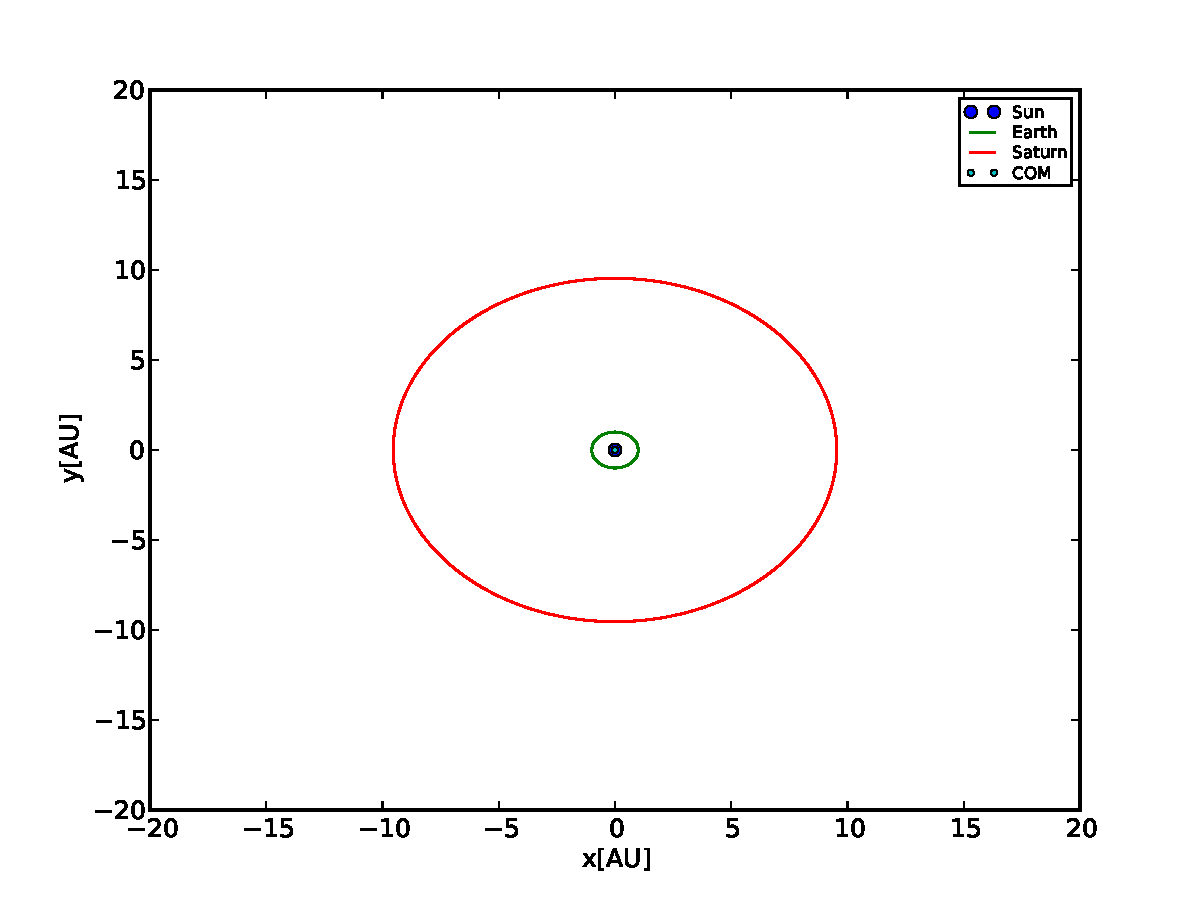
\includegraphics[width=\linewidth]{out}
	\caption{Sun in origin with Earth and Saturn in orbit.}
	\label{fig:simple}
\end{figure}
 For a 3-body system with the Sun, Earth and Saturn, the potential and kinetic energy did not change significantly over a period of 10 years
 (changes were of the order $10^{-6}$).

\section{Remarks}
The repository where you can find the programs is at \url{https://github.com/miktoki/FYS3150}.


Despite not being able to accomplish the specified task to a satisfactory degree, 
I did learn a lot about debugging, classes in C++ and was reminded of some good programming habits.

%\bibliographystyle{plain}
%\bibliography{refs}

%\printindex
\end{document}


